% ============================================================
%  WBS (Work Breakdown Structure) — Phase 2 : Planification
%  Time'Eats — Cellule PMO
%  Projet : Refonte Web
% ============================================================
\documentclass[11pt,a4paper,oneside]{report}
\usepackage{../../style/consulting}
\usepackage{pdflscape}
\usepackage{graphicx}
\hypersetup{pdftitle={WBS — Refonte Web — Time'Eats PMO}}
\pagestyle{fancy}\fancyhf{}
\renewcommand{\headrulewidth}{0pt}
\fancyhead[L]{\begin{tikzpicture}[remember picture,overlay]
  \draw[cnNavy,line width=0.5pt](0,0)--(\textwidth,0);
\end{tikzpicture}\vspace{2pt}\timeeatslogo\hspace{4pt}\small\textcolor{cnSlate}{Time'Eats \textbf{·} WBS --- \textit{Refonte Web}}}
\fancyhead[R]{\small\textcolor{cnSlate}{\thepage}}
\fancyfoot[C]{\tiny\textcolor{cnSlate}{Document confidentiel --- Cellule PMO --- CESI MAALSI 2026}}
\begin{document}\small

\begin{center}
{\LARGE\bfseries\color{cnNavy} Work Breakdown Structure (WBS)}\\[4pt]
\textcolor{cnOrange}{\rule{10cm}{1pt}}\\[4pt]
{\large\color{cnSlate} Phase 2 --- Planification \quad|\quad Projet : \textbf{Refonte Web}}
\end{center}

\vspace{6pt}

\begin{finding}
Le WBS décompose l'intégralité du périmètre Refonte Web en \textbf{8 lots de travaux} (Work Packages) répartis sur \textbf{5 phases du cycle de vie}. Chaque lot est assigné à un responsable unique. La somme des lots = 100\,\% du périmètre, soit \textbf{\textasciitilde 480 jours-homme} cumulés (interne + ESN Sopra Steria au forfait).
\end{finding}

\vspace{6pt}

\section*{1 --- Vue tabulaire}

\begin{landscape}
\scriptsize
\renewcommand{\arraystretch}{1.1}
\begin{tabularx}{\linewidth}{C{1.6cm} L{6cm} Y C{3cm} C{1.6cm}}
\toprule
\rowcolor{cnNavy}
\th{Code WBS} & \th{Livrable / Lot de travaux} & \th{Description} & \th{Responsable} & \th{Charge (j.h)} \\
\midrule

\multicolumn{5}{l}{\cellcolor{cnNavy!15}\textbf{\textcolor{cnNavy}{1. Démarrage}}} \\
\midrule
1.1 & Note de cadrage approuvée   & Périmètre, objectifs, options & CP (M. X)      & 4 \\
\rowcolor{cnIce}
1.2 & Charte projet signée        & Autorisation officielle DSI + DG & CP                  & 3 \\
1.3 & Équipe projet staffée       & Lettres de mission, contrat ESN  & CP + DSI            & 5 \\
\rowcolor{cnIce}
1.4 & Kick-off réalisé            & Lancement formel J0 le 22/04/2026 & CP                  & 2 \\
\midrule

\multicolumn{5}{l}{\cellcolor{cnNavy!15}\textbf{\textcolor{cnNavy}{2. Planification}}} \\
\midrule
2.1 & PMP validé (ce document)    & Plan de Management Projet baseline & CP + PMO            & 8 \\
\rowcolor{cnIce}
2.2 & WBS \& PBS                  & Décomposition produit + travaux   & CP + Tech Lead      & 4 \\
2.3 & Planning Gantt baseline     & 18 semaines, chemin critique      & CP + ESN            & 5 \\
\rowcolor{cnIce}
2.4 & Budget détaillé             & 300 K€ ventilés par poste         & CP + Contrôle gestion & 4 \\
2.5 & Registre risques v1         & 7 risques cotés, mitigation       & CP + RSSI           & 3 \\
\rowcolor{cnIce}
2.6 & Plan communication + comm.\ changement & Matrice + actions ADKAR    & CP + Marketing      & 4 \\
\midrule

\multicolumn{5}{l}{\cellcolor{cnNavy!15}\textbf{\textcolor{cnNavy}{3. UX/UI \& Design System}}} \\
\midrule
3.1 & Audit UX / parcours utilisateurs  & Heuristiques, analyse data analytics & UX Designer (Mme C) & 12 \\
\rowcolor{cnIce}
3.2 & Wireframes \& prototypes interactifs & 10 templates, Figma           & UX Designer + ESN   & 25 \\
3.3 & Design System v1                   & Tokens, composants, doc Storybook & UX + Tech Lead     & 18 \\
\rowcolor{cnIce}
3.4 & Validation maquettes (J1)          & Workshops MOA + tests utilisateurs & UX + MOA Marketing  & 8 \\
\midrule

\multicolumn{5}{l}{\cellcolor{cnNavy!15}\textbf{\textcolor{cnNavy}{4. Socle technique \& API}}} \\
\midrule
\rowcolor{cnIce}
4.1 & Architecture cible documentée & Diagrammes C4, ADR, choix stack   & Tech Lead (M. A) & 8 \\
4.2 & API REST v1 (OpenAPI 3)       & Catalogue, recherche, contact, comptes & ESN Sopra Steria + Dev Back (M. B) & 55 \\
\rowcolor{cnIce}
4.3 & Pipeline CI/CD multi-env.     & GitHub Actions, ARM templates, dev/staging/prod & DevOps (M. D) & 12 \\
4.4 & Socle SSO Office 365 (ou repli IdP local) & Authentification espace client & Tech Lead + RSSI    & 10 \\
\rowcolor{cnIce}
4.5 & Socle validé (J2)             & Recette socle, démonstration COPIL & Tech Lead           & 3 \\
\bottomrule
\end{tabularx}

\newpage
\renewcommand{\arraystretch}{1.1}
\begin{tabularx}{\linewidth}{C{1.6cm} L{6cm} Y C{3cm} C{1.6cm}}
\toprule
\rowcolor{cnNavy}
\th{Code WBS} & \th{Livrable / Lot de travaux} & \th{Description} & \th{Responsable} & \th{Charge (j.h)} \\
\midrule

\multicolumn{5}{l}{\cellcolor{cnNavy!15}\textbf{\textcolor{cnNavy}{5. Réalisation produit}}} \\
\midrule
5.1 & Site corporate (10 templates Next.js) & Pages publiques + SEO technique & ESN front + Tech Lead & 80 \\
\rowcolor{cnIce}
5.2 & CMS contributeur \& workflows éditoriaux & Création contenu, médias, SEO, workflow validation & ESN + Marketing & 45 \\
5.3 & Espace client (compte, commandes, factures) & Parcours authentifié & ESN front/back   & 55 \\
\rowcolor{cnIce}
5.4 & Intégrations (analytics, monitoring APM, paiement v0) & GA4, Application Insights, Stripe sandbox & DevOps + ESN    & 18 \\
5.5 & MVP en staging (J3)           & Démo MOA, recette interne        & CP + ESN            & 4 \\
\midrule

\multicolumn{5}{l}{\cellcolor{cnNavy!15}\textbf{\textcolor{cnNavy}{6. Qualité \& Recette}}} \\
\midrule
6.1 & Tests unitaires \& d'intégration   & Couverture $\geq$ 80\,\% (Vitest, Jest) & ESN + Tech Lead     & 20 \\
\rowcolor{cnIce}
6.2 & Audit accessibilité RGAA 4.1 AA    & Audit externe + corrections    & ESN UX + audit ext. & 12 \\
6.3 & Audit sécurité OWASP ASVS 2        & Pentest + corrections critiques & RSSI + audit ext.  & 15 \\
\rowcolor{cnIce}
6.4 & Tests perf (Lighthouse, charge k6) & Web Vitals + charge cible      & DevOps + Tech Lead  & 8 \\
6.5 & Recette fonctionnelle MOA + PV (J4) & Cahier de tests, PV signé      & CP + MOA            & 10 \\
\midrule

\multicolumn{5}{l}{\cellcolor{cnNavy!15}\textbf{\textcolor{cnNavy}{7. Conduite du changement}}} \\
\midrule
7.1 & Communication interne (sensibilisation) & Newsletter, intranet, démos & CP + Marketing      & 6 \\
\rowcolor{cnIce}
7.2 & Formation contributeurs CMS (Key Users) & 4 sessions, 12 contributeurs & CP + ESN + Marketing & 8 \\
7.3 & Documentation utilisateur (FAQ, guides) & Espace SharePoint dédié    & CP + Support        & 6 \\
\midrule

\multicolumn{5}{l}{\cellcolor{cnNavy!15}\textbf{\textcolor{cnNavy}{8. Clôture \& Go-Live}}} \\
\midrule
8.1 & Bascule production (J5) & DNS, certificats, monitoring run & DevOps + Tech Lead  & 5 \\
\rowcolor{cnIce}
8.2 & Hypercare M+1           & Support renforcé, hotline DSI    & CP + DSI Ops        & 8 \\
8.3 & Transfert exploitation  & Documentation run, formation équipe DSI Ops & CP + DSI Ops & 5 \\
\rowcolor{cnIce}
8.4 & Fiche REX + clôture     & Capitalisation PMO, archivage    & CP + PMO            & 4 \\

\midrule
\rowcolor{cnNavy!10}
\multicolumn{4}{l}{\textbf{TOTAL projet (interne + ESN forfait 400 j.h)}} & \textbf{\textasciitilde 480 j.h} \\
\bottomrule
\end{tabularx}
\end{landscape}

\vspace{4pt}

\section*{2 --- Vue graphique (arborescence)}

\begin{center}
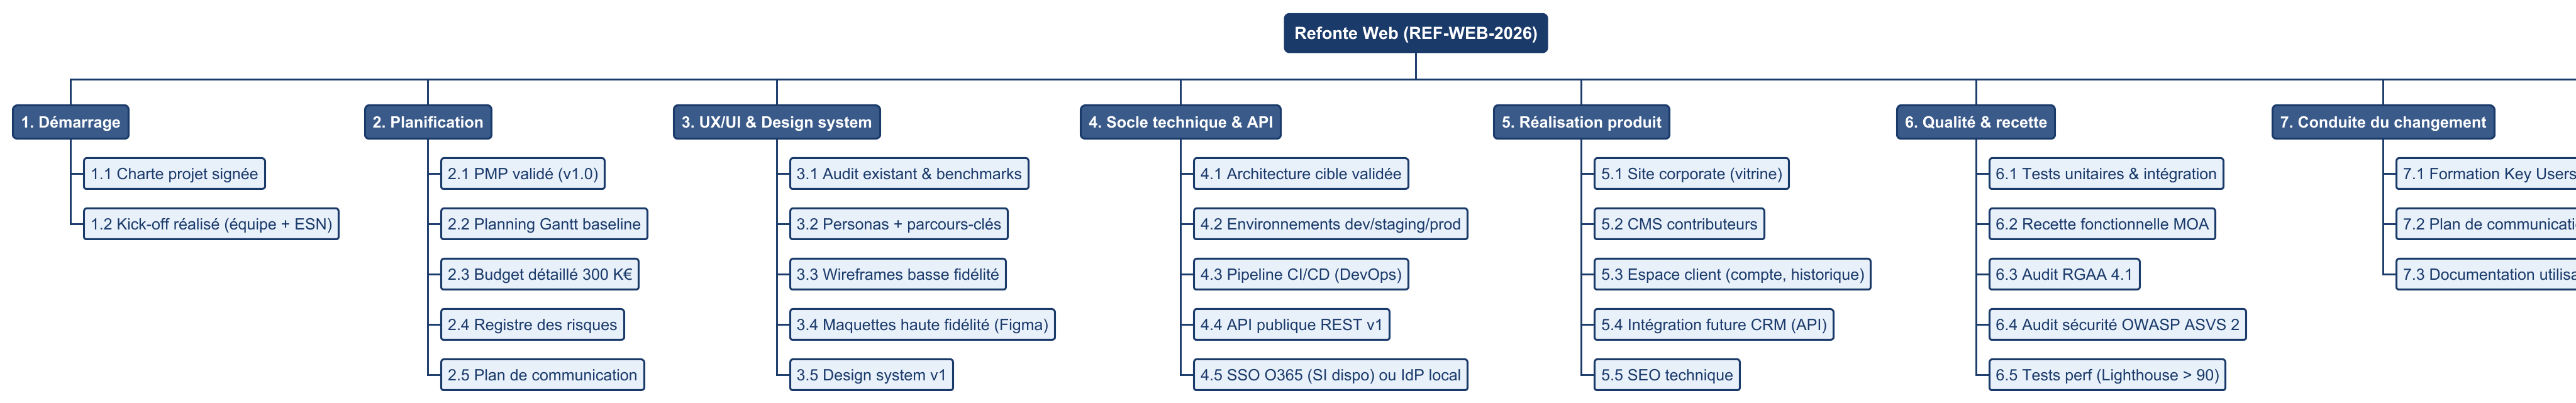
\includegraphics[width=\textwidth,keepaspectratio]{../../diagrammes/wbs_refonte_web.png}
\end{center}

\vspace{4pt}

\begin{reco}
\textbf{Règles de gestion du WBS :}
\begin{itemize}
  \item La version de référence (baseline) est celle validée au COPIL d'inception du \textbf{20/05/2026}.
  \item Tout écart $>$ 5\,\% sur la charge d'un lot doit déclencher un \textbf{rapport d'écarts}.
  \item Toute demande de changement de périmètre fait l'objet d'un \textbf{avenant} validé en COPIL avant intégration au WBS.
  \item Le WBS est mis à jour mensuellement par le CP ; le PMO archive chaque version dans SharePoint.
\end{itemize}
\end{reco}

\end{document}
